\chapter{Popular CNN Models}

\section{LeNet/ LeNet-5 (1998) \cite{gfg-convolutional-neural-network-cnn-in-machine-learning,wiki-lenet,ieee/726791/cnn-lenet,medium/lenet-5-complete-architecture-84c6d08215f9}}\label{cnn: LeNet}

\begin{figure}[h]
    \centering
    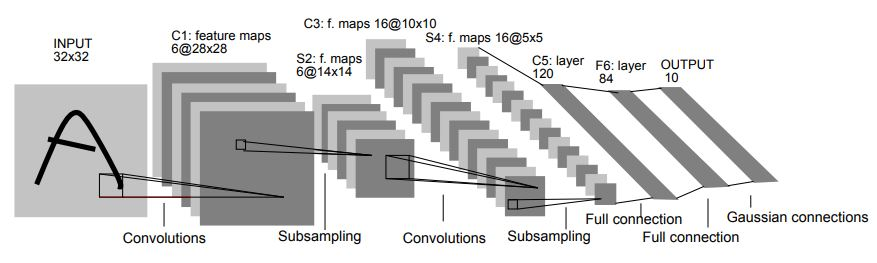
\includegraphics[width=\linewidth, height=5cm, keepaspectratio]{Pictures/convolutional-neural-network/LeNet_Original_Image.jpg}
    \caption{CNN: LeNet}
\end{figure}

\begin{itemize}
    \item LeNet is a convolutional neural network structure proposed by LeCun et al. in 1998. \cite{ieee/726791/cnn-lenet}
    
    
    \item In general, LeNet refers to LeNet-5 and is a simple convolutional neural network.
\end{itemize}


\begin{longtable}{|>{\centering\arraybackslash}m{1.5cm}|>{\centering\arraybackslash}m{2cm}|>{\centering\arraybackslash}m{1.5cm}|>{\centering\arraybackslash}c|>{\centering\arraybackslash}m{1cm}|>{\centering\arraybackslash}m{1.5cm}|>{\centering\arraybackslash}m{2cm}|>{\centering\arraybackslash}m{2cm}|}
    \caption{CNN: LeNet-5 Architecture \cite{medium/lenet-5-complete-architecture-84c6d08215f9}}\\

    \hline
    \textbf{Layer No.} & \textbf{Layer} & \textbf{Feature Map} & \textbf{Size} & \textbf{Kernel Size} & \textbf{Stride} & \textbf{Activation} & \textbf{Trainable Params} \\
    \hline
    \endfirsthead

    \hline
    \textbf{Layer No.} & \textbf{Layer} & \textbf{Feature Map} & \textbf{Size} & \textbf{Kernel Size} & \textbf{Stride} & \textbf{Activation} & \textbf{Trainable Params} \\
    \hline
    \endhead

    \hline\endfoot
    \hline\endlastfoot

    Input & Image & 1 & $32\times 32$ & - & - & - & - \\
    \hline

    1 & Convolution & 6 & $28\times 28$ & $5\times 5$ & 1 & tanh & 156 \\
    \hline

    2 & Average Pooling & 6 & $14\times 14$ & $2\times 2$ & 2 & tanh & 0 \\
    \hline

    3 & Convolution & 16 & $10\times 10$ & $5\times 5$ & 1 & tanh & 2416 \\
    \hline

    4 & Average Pooling & 16 & $5\times 5$ & $2\times 2$ & 2 & tanh & 0 \\
    \hline

    5 & Convolution & 120 & $1\times 1$ & $5\times 5$ & 1 & tanh & 48120 \\
    \hline

    6 & FC & - & 84 & - & - & tanh & 10044 \\
    \hline

    Output & FC & - & 10 & - & - & softmax & 850 \\
    \hline
\end{longtable}


\begin{lstlisting}[language=Python,title=LeNet - tensorflow - Python]
import tensorflow as tf
from tensorflow.keras import layers, models

# Define the model
model = models.Sequential()

# Layer 1: Convolutional Layer
model.add(
    layers.Conv2D(6, (5, 5), 
    activation='tanh', 
    input_shape=(32, 32, 1))
)

# Layer 2: Average Pooling
model.add(layers.AveragePooling2D((2, 2)))

# Layer 3: Convolutional Layer
model.add(layers.Conv2D(16, (5, 5), activation='tanh'))

# Layer 4: Average Pooling
model.add(layers.AveragePooling2D((2, 2)))

# Layer 5: Convolutional Layer
model.add(layers.Conv2D(120, (5, 5), activation='tanh'))

# Flatten the tensor
model.add(layers.Flatten())

# Layer 6: Fully Connected Layer
model.add(layers.Dense(84, activation='tanh'))

# Output Layer: Fully Connected Layer
model.add(layers.Dense(10, activation='softmax'))

# Print the model summary
model.summary()
\end{lstlisting}

\textbf{Output}:
\begin{lstlisting}[numbers=none]
Model: "sequential"
_________________________________________________________________
 Layer (type)                Output Shape              Param #   
=================================================================
 conv2d (Conv2D)             (None, 28, 28, 6)         156
 average_pooling2d (Average  (None, 14, 14, 6)         0
 Pooling2D)
 conv2d_1 (Conv2D)           (None, 10, 10, 16)        2416
 average_pooling2d_1 (Avera  (None, 5, 5, 16)          0
 gePooling2D)
 conv2d_2 (Conv2D)           (None, 1, 1, 120)         48120
 flatten (Flatten)           (None, 120)               0
 dense (Dense)               (None, 84)                10164
 dense_1 (Dense)             (None, 10)                850
=================================================================
Total params: 61706 (241.04 KB)
Trainable params: 61706 (241.04 KB)
Non-trainable params: 0 (0.00 Byte)

\end{lstlisting}


\url{https://medium.com/codex/lenet-5-complete-architecture-84c6d08215f9}







\section{AlexNet \cite{gfg-convolutional-neural-network-cnn-in-machine-learning}}\label{cnn: AlexNet}











\section{ResNet \cite{gfg-convolutional-neural-network-cnn-in-machine-learning}}\label{cnn: ResNet}
















\section{GoogleNet \cite{gfg-convolutional-neural-network-cnn-in-machine-learning}}\label{cnn: GoogleNet}














\section{MobileNet \cite{gfg-convolutional-neural-network-cnn-in-machine-learning}}\label{cnn: MobileNet}















\section{VGG \cite{gfg-convolutional-neural-network-cnn-in-machine-learning}}\label{cnn: VGG}













































